%!TEX root = ../report.tex
\chapter{Hardware Architecture}
\label{ch:hardware}
This section describes the hardware architecture of \ProjectName{}. The description will be more high-level along with explanation about the hardware platform and the application interfaces between each components of the system. The rest of this chapter is organized as follows. First section, \autoref{sec:hardware-overview}, presents an overview of the hardware implemented in this system depicted in big schema. Decisions made in this system are detailed in \autoref{sec:hardware-decisions} with tables. Lastly, hardware description is described in \autoref{sec:hardware-description}.

\section{Hardware Overview}
\label{sec:hardware-overview}
The \ProjectName{} hardware components can be categorized into four main components: sensing part, data storing part, analytics part, and data presentation part. The data flow starts from wired and wireless sensors located across the Netherlands that collects information for monitoring. The process will end at data presentation and warning dispatch in the users' side. The overview of the hardware and its application interfaces are depicted in \autoref{fig:hardware-archi-schema} below.

% btw is it suppose to be the other way around? sensor monitoring -> analytics-> database ?
\begin{figure}[hb!]
\centering
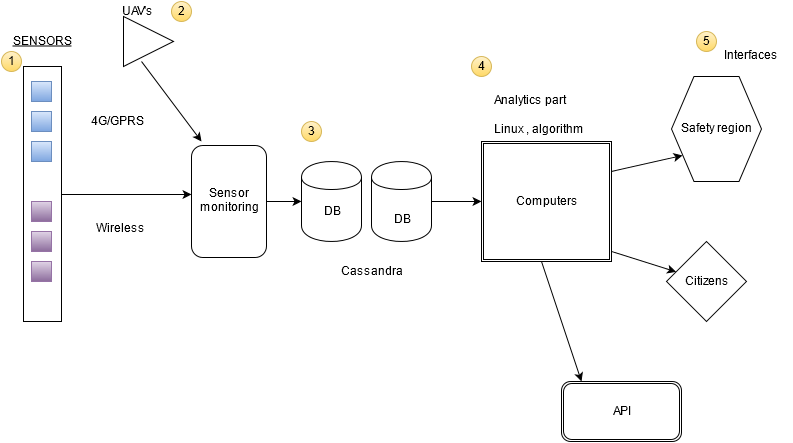
\includegraphics[scale=0.5]{images/HardwareArchitectureOverview.png}
\caption{Schematic overview of the hardware architecture of \ProjectName{}}
\label{fig:hardware-archi-schema}
\end{figure}

Here is an overview of the Hardware Architecture. Each number corresponds to a decision which will be detailed in the Hardware Design Decision part.

The \ProjectName{} will utilize wired and wireless sensor for monitoring water ways and dikes. Wired sensor will be placed in congested dikes and waterways where wired connection is possible. Wireless sensor will be planted in remote areas where wired connections are impossible or too costly. UAVs will fly to check reported faulty sensors. UAVs will also be used to take required pictures for further analytics or to examine some portion of the system which is hard or impossible for a personnel to access. Then all measurement will be forwarded to sensor monitoring part to be normalized before getting in to the analytics part.

The next part of the hardware is the cluster for carrying out analysis. This will be a collection of servers that is coordinated using clusters. This part also handles the logic for detecting faulty sensors, as the sensor monitoring parts contain no logic behind it.

SFM will use other cluster to store our important data. This cluster will run Cassandra database on top if it. This cluster will also have several interfaces to communicate with other instances, such as main analytics part, third party data gathering cluster, and API cluster.

The last part of the hardware architecture is third party data gathering cluster and API cluster. Third party data gathering cluster is responsible for collecting weather forecast and demographic information of the Netherlands. Meanwhile, API cluster is responsible for handling request from actors that will consume our practical information and for notifying safety region in case of imminent flood. Both of this cluster are merely collections of server computer that works together.

\section{Hardware Design Decisions}
\label{sec:hardware-decisions}
This section defines decisions made regarding the hardware selection. Tables will be used to make our justification in regard to hardware selection more crystal clear.

\begin{table}[h!]
\begin{tabular}{L{0.2\textwidth} L{0.6\textwidth}}
    \textbf{Name} 			& \textbf{Choice of the computer for data analyze} \\ \toprule
    \textbf{Decision} 		& \textbf{DEC-4}\\ \midrule
    \textbf{Status} 		& \textbf{Approved} \\ \midrule
    \textbf{Problem/Issue} 	& The system needs computer to analyze data from sensors, UAV's ,weather forecast. \\ \midrule
    \textbf{Decision} 		& IBM Supercomputer ...\\ \midrule
    \textbf{Alternatives} 	& \textit{BB}\\
    						& Other brand .\\
    						& \textit{BB}\\
    						& BBBB.\\
    						\midrule
    \textbf{Arguments} 		& IBM supercomputer uses Linux which is the oS we choosed. \\
    						& 	\begin{tabular}{l|lllllll|l}
							& 		\rot{Reliability} & \rot{Resilience} & \rot{Performance} & \rot{Security} & \rot{Scalability} & \rot{Cost} & \rot{\textbf{Score}} \\ \hline
							% 					
								\end{tabular} \\
    \\ \bottomrule
\end{tabular}


IBM supercomputer uses Linux which is the oS we chose.

\caption{Decision -- Choice of computer}
\label{table:linux}
\end{table}

%Performance , Speed of calculation , Core ; lINUX

\begin{table}[h!]
\begin{tabular}{L{0.2\textwidth} L{0.6\textwidth}}
    \textbf{Name} 			& \textbf{Data representation - Interface with the third parties} \\ \toprule
    \textbf{Decision} 		& \textbf{DEC-4}\\ \midrule
    \textbf{Status} 		& \textbf{Approved} \\ \midrule
    \textbf{Problem/Issue} 	& The system needs to interact with the third parties. \\ \midrule
    \textbf{Decision} 		& Dashboard for the emergency services\\ Rack server \\ \midrule
    \textbf{Alternatives} 	& \textit{BB}\\
    						& DRAFT .\\
    						& \textit{BB}\\
    						& BBBB.\\
    						\midrule
    \textbf{Arguments} 		& \\

    \\ \bottomrule
\end{tabular}
\caption{Decision -- Interface with third parties}
\label{table:linux}
\end{table}



% ng180levee
\begin{table}[h!]
\begin{tabular}{L{0.2\textwidth} L{0.6\textwidth}}
    \textbf{Name}           & \textbf{Choice of dike sensor} \\ \toprule
    \textbf{Decision}       & \textbf{3}\\ \midrule
    \textbf{Status}         & \textbf{Approved} \\ \midrule
    \textbf{Problem/Issue}  & The system needs a reliable sensor system to measure condition of dikes. \\ \midrule
    \textbf{Decision}       & The system will implement GeoBeads MEMS Sensor in water ways and dikes.\\ \midrule
    \textbf{Alternatives}   & \textit{GeoBeads}\\
                            & The GeoBead is a compact sensor, which can measure the pore pressure, temperature and local tilt in dikes. A unit costs about 350 dollar\cite{ng180levee}. \\
                            & \textit{Piezometers}\\
                            & Piezometers measure the pore water pressure in the dikes. This information can be used to measure the stability of the dike. A piezometer costs about 200 dollar\cite{ng180levee}. \\
                            & \textit{Volt meters} \\
                            & Volt meters can be used to measure the streaming potential in the dike, which are an indicator of its stability\cite{selfpotential}. These sensors are approximately 50 dollars per unit. Materials in the dike can decrease the accuracy of this measurement technique. \\
                            \midrule
    \textbf{Arguments}      & \\
                            &   \begin{tabular}{l|lllllll|l}
                            &       \rot{Reliability} & \rot{Resilience} & \rot{Performance}& \rot{Interoperability} & \rot{Security} & \rot{Scalability} & \rot{Cost} & \rot{\textbf{Score}} \\ \hline
                            %                  rel res perf int sec sca cost
                                    GeoBeads   & 5 & 4 &  & 3 &    &   & 2 & 14\\ 
                                    Piezometer & 4 & 2 &  & 2 &    &   & 3 & 11\\
                                    Volt meters& 1 & 5 &  & 2 &    &   & 5 & 13\\
                                \end{tabular} \\
    \\ \bottomrule
\end{tabular}
\caption{Decision -- Choice of Sensors}
\label{table:linux}
\end{table}


% ng180levee
\begin{table}[h!]
\begin{tabular}{L{0.2\textwidth} L{0.6\textwidth}}
    \textbf{Name}           & \textbf{Connectivity of the dike sensor} \\ \toprule
    \textbf{Decision}       & \textbf{3}\\ \midrule
    \textbf{Status}         & \textbf{New} \\ \midrule
    \textbf{Problem/Issue}  & The dike sensors have to be connected to the internet in some way, so they can send their data to the central server. \\ \midrule
    \textbf{Decision}       & The sensors will be connected by a wire.\\ \midrule
    \textbf{Alternatives}   & \textit{Wired}\\
                            & A wired cable connects the dike sensor. This cable can also be used to supply the sensor with electricity. \\
                            & \textit{ZigBee}\\
                            & ZigBee is an open protocol for personal area networks. It uses little power and is therefore a good choice for devices equipped with a battery. \\
                            & \textit{ISM radio band} \\
                            & The ISM radio bands can be used for industrial, scientific and medical purposes.  \\
                            \midrule
    \textbf{Arguments}      & ZigBee is not an option, since the sensors are embedded in the soil of the dikes, and the frequency it uses, decreases too much in strength when traveling through the dike\cite{van2009draadloos}. \\
                            & Research has been done by van der Gees and Kok \cite{van2009draadloos} to determine if it is feasible to use the ISM radio band to communicate from within the dike. They concluded that, while it is possible to communicate through the dike using this band, the distance is limited and the rate of error is relatively high.
                            \\
                            & While a wire is not ideal in the sense that it will have to connect all the sensors, it seems to be the best option for the sensor in the dikes. It has the additional benefit that it can also supply the sensors with electricity.
    \\ \bottomrule
\end{tabular}
\caption{Decision -- Connectivity of the dike sensor}
\label{table:linux}
\end{table}


\clearpage
\section{Hardware Description}
\label{sec:hardware-description}
% Mention the difference between previous chapter
This section outlines describes description of the hardware implemented in this system. This section also supports decisions of hardware selection in previous section.

\subsection{Sensing Components}
\label{subsec:sensing-components}
Roughly 17.000 kilometers of dikes protect the Netherlands against flooding\cite{DMC}. Of this, about 3.500 kilometers are primary dikes\cite{waterwijzer}. These are dikes protecting against the water of the sea, the big rivers (Rijn, Maas, IJssel), the IJsselmeer and the Markermeer. 

The hardware architecture of the system is composed of two sensing components. The first sensing component are sensors installed in the dikes to measure and detect potential instability of the dikes.
The second sensing component consists of water level sensors, which are spread along water ways in the country, to measure the water level. 

\subsubsection{Dike sensors}
To measure the stability of the dikes, GeoBeads dike monitoring sensor will be installed in the dikes. When these sensors are placed in the dike with a spacing of 3 meters, they will provide optimal measurements\cite{ng180levee}.

The GeoBeads is embedded in the dike and is installed using conventional CPT push-in techniques. %Three sensors are installed per cross-section and a cross-section is installed every 100 m. Each CPT push-in costs about \EUR200 per sensor\cite{TUDelftPHD}.%pp126

The GeoBeads are connected by communication cable, which also functions as a power supply. 

\subsubsection{Water level sensors}

% Adds some picture here

\subsection{Database Cluster and Data Collection}
\label{subsec:database-data}
In the previous chapter, SFM will use Cassandra database as the database platform. However, Cassandra requires computers to run its environment. SFM will use clusters of computer to manage database system and to store our data. The cluster will also be accessible by other portions of our hardware, such as main analytics parts, third party data gathering part, and API part.

There are four servers and each server costs AC 1.500. To enhance the availability, the servers will be redundantly set up four times. Resulting in a hardware cost for the servers of
Server cost= 4 ∗ 1500 ∗ 4 = 24.000. The total hardware costs is shown in the table below.

Clustering, in the context of databases, refers to the ability of several servers or instances to connect to a single database. An instance is the collection of memory and processes that interacts with a database, which is the set of physical files that actually store data.

Clustering offers two major advantages, especially in high-volume database environments:

Fault tolerance: Because there is more than one server or instance for users to connect to, clustering offers an alternative, in the event of individual server failure.
Load balancing: The clustering feature is usually set up to allow users to be automatically allocated to the server with the least load.

% Adds some picture here

\subsection{Analytics Components}
\label{subsec:analytics}

% Server specs
% - Server
% - Networking device
% - UPS